%!TEX root = article.tex
\section{Experiments}\label{sec:exps}

\begin{figure*}[t]
    \centering
    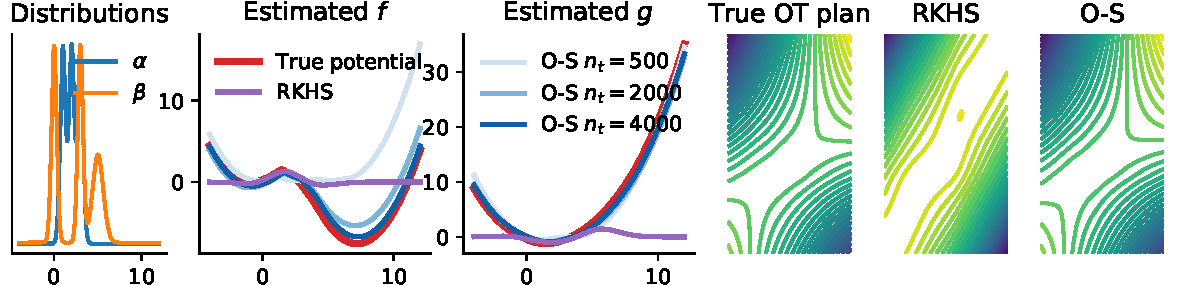
\includegraphics[width=\linewidth]{continuous.pdf}
    \caption{Representation of the convergence path of online Sinkhorn: the blue curves represents the estimated potentials (continuous functions) at different stage of the algorithm. The estimated plan $\pi_t$ is very quickly accurate, while the shape of the potentials match nearly perfectly the true potentials (estimated on a grid $N = 5000$).}
    \label{fig:potentials}
\end{figure*}


We have introduced and stated convergence results on the online Sinkhorn
algorithms. These convergence results are non-quantitative, and therefore
requires an extensive experiment validation. Our experiments will be three-fold:
first, we show that online Sinkhorn accurately estimates correctly the solutions
of \eqref{eq:wass} and the Sinkhorn distance, overcoming the bias due to
sampling only once in the regular Sinkhorn algorithm. Then, we show
how online Sinkhorn can accelerate the Sinkhorn algorithm, by estimating sketches
of potentials simultaneously to the computation of the distance matrix. Finally, we show
how online Sinkhorn allows to estimate potentials with accurate shapes, compared
to SGD with RKHS representations \citep{2016-genevay-nips}.

\subsection{Consistent estimation of Sinkhorn distances}

We first work with discrete probabilities $(\alpha, \beta)$, to be able to compute a reference
distance $\Ww(\alpha, \beta)$ and potentials $f^\star$, $g^\star$, using the Sinkhorn
algorithm. We note that we do not hope to perform better than the Sinkhorn
algorithm, as the constraint of online Sinkhorn yields unnecessary slow-downs in
this case---instead, our purpose is simply to show the consistence of online
Sinkhorn. We choose $\alpha$ and $\beta$ to be two simple discrete $1D$
distributions, sampled from the one displayed in \autoref{fig:potentials}. We set
$\varepsilon = 10^{-2} \max_{x,y} C(x,y)$. We
compare the performance of Sinkhorn, online Sinkhorn and random Sinkhorn,
measuring $\Vert f - f^\star \Vert_{\text{var}} + \Vert g - g^\star
\Vert_{\text{var}}$ and the absolute error $| \Ww_t - \Ww |$ versus the number
of computations performed--- the evaluation of $C(x_i, y_i)$ and the computation
of each addition in the $C$-transform are elementary computation units.
Additionaly, we report the curves using out-of-loop averaging. 

\begin{figure}[t]
    \centering
    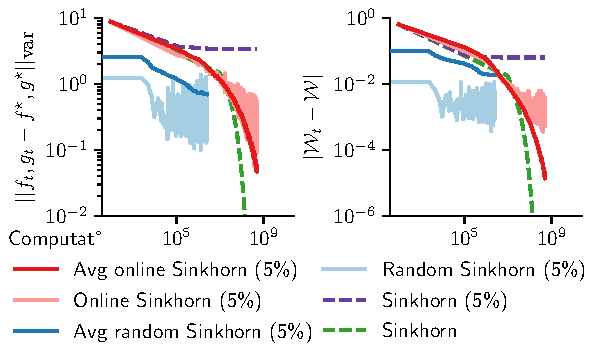
\includegraphics[width=\linewidth]{comparison.pdf}
    \caption{Comparison of online, random and fixed sampling Sinkhorn performances. Online Sinkhorn overcome the bias of sampling---especially with out-of-loop averaging. Random Sinkhorn gives fast estimations, whose variance do not decrease.}
    \label{fig:convergence}
\end{figure}

\paragraph{Results.} We report convergence curves in \autoref{fig:convergence}.
Compared to the subsampled Sinkhorn algorithm that computes a biased estimate of
the distance $\Ww$ (purple), the online Sinkhorn algorithm successfully
estimates the distance and the associated potentials, despite performing only
partial $C$-transforms (green). Random Sinkhorn (red) finds a decent estimation
of the distance and potentials, with fewer computations than the full Sinkhorn
algorithm, but fails to converge. Averaging the random Sinkhorn iterations finds
a biased estimation. The vanilla online Sinkhorn converges towards the true
value, albeit with a rather high iterate variance (note that this variance does
reduce---this is a log-log plot). Remarkably, the out-of-loop averaging of
online Sinkhorn enjoys much better converging property---we confirmed this
finding on many synthetic problems. It is surprising that an averaging mechanism
brings speed-up in a non-convex setting---we attribute this to the convexity of
the original problem, although this should be further investigated.

\begin{figure}[t]
    \centering
    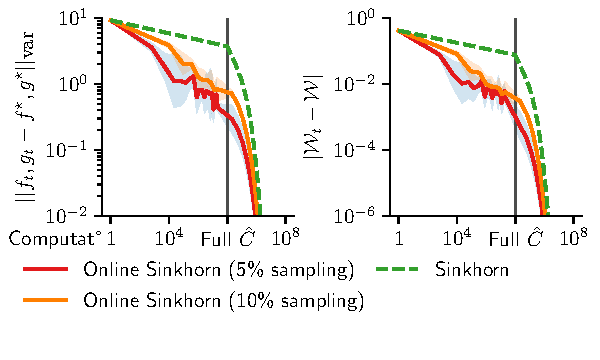
\includegraphics[width=\linewidth]{early_compute}
    \caption{Using online Sinkhorn during the initial computation of the cost
     matrix brings a significant speed-up to the Sinkhorn algorithm: it provides
     good estimates of the potentials $f_t$ and $g_t$ usable as initializaiton
     for the first full Sinkhorn iteration. Curves averaged over 5 runs. \label{fig:early_compute}}
\end{figure}

\subsection{Accelerating the first Sinkhorn iteration}\label{sec:accelerating}

The Sinkhorn algorithm requires to compute the matrix $C$ prior to estimating
the first potentials $f_1$ and $g_1$. Online Sinkhorn jointly computes this
matrix with first sketches of the potentials. We therefore assess the
performance of the following \textit{online+full Sinkhorn} algorithm in a
discrete setting: online Sinkhorn is run for the first $n_t$ iterations, until
the cost matrix $C$ is completely evaluated. At this point (iteration $t$),
online Sinkhorn provides the estimates $f_{t}, g_{t}$. From then, the algorithm
only performs full Sinkhorn updates.

\paragraph{Results.} We report convergence curves in
\autoref{fig:early_compute}. The proposed scheme indeed provides an improvement
upon Sinkhorn algorithm. After $N^2$ computation (the cost of estimating $C$),
both the function value and distance to optimum are lower using our scheme: the
Sinkhorn algorithm can operate on initial good approximations of optimal
potentials, provided for approximately twice the cost of estimating the matrix
$C$ in dimension $1$. The \textit{online+full} Sinkhorn algorithm thus keep an
advantage over the full Sinkhorn algorithm over time. Note that the cost of
estimating these potentials becomes negligible as the dimension increase---the
cost of computing $C$ dominates. This strongly advocates for using an online
scheme as a warm-up for regularized OT estimation. The gain decrease with
$\epsilon$, but remains important even for $\epsilon = 10^{-4} \max C$ (see
appendix). We add that using a
sampling-without-replacement scheme brings an additional speed-up (see appendix), as well as out-of-loop averaging.

\subsection{Continuous potential estimation}

Finally, we measure the performance of our algorithm in a truly continuous
setting, where $\alpha$ and $\beta$ are parametric distributions (Gaussian
mixtures) from which we sample. In the absence of reference $\Ww$ (which is
precisely not computable without a method akin to ours), we monitor the
trajectories of the potentials, and compare them to the Sinkhorn potentials for
realisation of $\alpha$ and $\beta$ of size $n=2000$. We also monitor the
estimated transportation plan $\hat \pi_t = \alpha \otimes \beta
\exp(\frac{f\oplus g - C}{\varepsilon})$. We run the experiments with
$n_t=5000$.

\paragraph{Results.} We show the convergence trajectories of the potentials in
\autoref{fig:potentials}. Online Sinkhorn refines the potentials $(f_t, g_t)_t$ until convergence. Our usage of the natural potential parametrization \eqref{eq:param}
allows the iterates to quickly identify the correct function shape. The final
plan is undistinguishable from the true transportation plan. Quantitative values
converge similarly to the curves in \autoref{fig:convergence}.

\paragraph{Comparison to concurrent approach.} Finally, we compare online
Sinkhorn to constructing representations of Sinkhorn potentials in universal
RKHS \cite{2016-genevay-nips}. This competing approach sets $f_t(\cdot) =
\sum_{i=1}^{n_t} \alpha_t \kappa(\cdot, x_i)$, with similar $g_t$, where $\kappa$ is
a reproducing kernel (typically a Gaussian). This differs from the
representations that we propose, for which $\exp(-f_t)$, and not $f_t$, is
expressed as a Gaussian mixture. With RKHS representations of potentials, the
dual problem \eqref{eq:sinkhorn} can be solved using stochastic gradient
descent, with theoretical convergence guarantees. As advocated by the authors,
we run a grid over the bandwidth parameter $\sigma$ to select the best
performing runs. We set $n_t = 50000$, and $\epsilon = 10^{-1} \max C$. We could not successfully use the method for lower $\epsilon$.

We compare the final potentials and associated
transportation plans in \autoref{fig:comparison_rkhs}. Our method estimates
potentials with much less errors, especially in areas where the mass of $\alpha$
and $\beta$ is low. Its computational complexity is comparable. Furthermore, it
does not require to set any hyperparameters, whereas we observed RKHS SGD to be
very sensitive to bandwidth selection.

\begin{figure}[t]
    \centering
    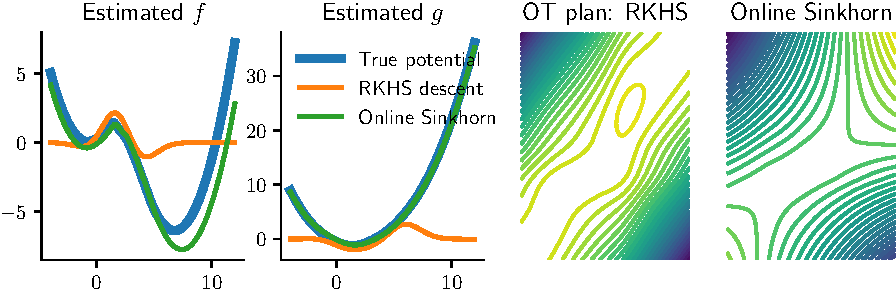
\includegraphics[width=\linewidth]{continuous_francis-crop.pdf}
    \caption{Comparing online Sinkhorn with SGD over a RKHS representation of the potential \citep{2016-genevay-nips}, with best bandwidth parameter. Online Sinkhorn finds more accurate functional representations of potentials, thanks to its more appropriate parametrization.}
    \label{fig:comparison_rkhs}
\end{figure}